\documentclass{cours}
\usepackage{pgfplots}
\usepackage{multicol}
\usepackage{cases}
\usepackage{amssymb}
\usepackage{calc}
%\usepackage{esvect}
\usepackage{tikz-3dplot} 
\usetikzlibrary{patterns}
\usetikzlibrary{decorations.text}

\begin{document}
\setcounter{chapter}{13}
\chapter{Moment cinétique et solides en rotation}
\section{Mouvements d'un solide}%
\label{sec:mouvements_d_un_solide}

\subsection{Définition}%
\label{sub:definition}

\begin{definition}
  Un solide est un ensemble de points matériels. On dit que le solide est indéformable si la distance entre chacun des points qui le composent est constante. Dans la suite, on se limitera à l'étude de solides indéformables.
\end{definition}

\subsection{Mouvements de translation}%
\label{sub:mouvements_de_translation}

\subsubsection{Translation rectiligne}%
\label{ssub:translation_rectiligne}

\begin{definition}
  On dit qu'un solide est en translation rectiligne, si chacun des points qui le composent a une mouvement de translation rectiligne. Tous le points du solide ont la même vitesse $\vv{v}$. 
\end{definition}

  \newcommand{\objet}[1]{
    \draw[thick, fill=white, fill opacity=0.8] #1 to[out=180, in=-90] ++(-1, 2) to[out=90, in=180] ++(1,1) to[out=0, in=90] ++(2,-1) to[out=-90, in=0] ++(-1,-1) to[out=180, in=0] ++(-1,-1);
    \draw[fill=black] ($#1+(0, 0.5)$) circle(2pt);
    \draw[fill=black] ($#1+(-0.5, 1.5)$) circle(2pt);
    \draw[fill=black] ($#1+(1.5, 2)$) circle(2pt);
    }

\begin{center}
  \begin{tikzpicture}[scale=0.7]
    \foreach \x in{0.5,1,...,6}{
    \pgfmathsetmacro{\opa}{0.4*\x/6}
    \begin{scope}[opacity=\opa]
     \objet{(\x,0)}
    \end{scope}
    }
    \objet{(6.5,0)}
    \draw[dashed, thin] (0, 0.5) -- (6.5, 0.5);
    \draw[dashed, thin] (-0.5, 1.5) -- (6, 1.5);
    \draw[dashed, thin] (1.5, 2) -- (8, 2);
  \end{tikzpicture}
\end{center}

\subsubsection{Translation circulaire}%
\label{ssub:translation_circulaire}

\begin{definition}
  Un solide est en translation circulaire lorsque tous ses points ont un mouvement circulaire de même rayon $r$. Le solide conserve une orientation fixe. Tous les points du solide ont le même vecteur vitesse $\vv{v} = r \dot{\theta}\vet$.  
\end{definition}

\begin{center}
  \begin{tikzpicture}[scale=0.7]
    \foreach \a in {10,30,...,340}{
    \pgfmathsetmacro{\opa}{0.6*\a/340}
    \begin{scope}[opacity=\opa]
    \objet{(\a:2)}
    \end{scope}
    }
    \objet{(0:2)}
    \draw[thin, dashed] (0, 0.5) circle(2);
    \draw[thin, dashed] (-0.5, 1.5) circle(2);
    \draw[thin, dashed] (1.5, 2) circle(2);
  \end{tikzpicture}
\end{center}

\subsection{Rotation autour d'un axe fixe}%
\label{sub:rotation_autour_d_un_axe_fixe}

\begin{definition}
  On dit qu'un solide est en rotation autour d'un axe fixe $\Delta$ lorsque tous ses points décrivent un mouvement circulaire autour de l'axe $\Delta$ à la même vitesse angulaire $\dot{\theta}$.  
\end{definition}

\begin{center}
\begin{tikzpicture}[scale=0.7]
    \foreach \a in {10,30,...,340}{
    \pgfmathsetmacro{\opa}{0.6*\a/340}
    \begin{scope}[opacity=\opa, rotate=\a]
    \objet{(2, 0)}
    \end{scope}
    }
    \objet{(0:2)}
    \pgfmathsetmacro{\r}{sqrt(2^2+0.5^2)}
    \draw[thin, dashed] (0, 0) circle(\r);
    \pgfmathsetmacro{\r}{sqrt(1.5^2+1.5^2)}
    \draw[thin, dashed] (0, 0) circle(\r);
    \pgfmathsetmacro{\r}{sqrt(3.5^2+2^2)}
    \draw[thin, dashed] (0, 0) circle(\r);
\end{tikzpicture}
\end{center}

La vitesse d'un point $M$ situé à une distance $r$ de l'axe est $\vv{v}=r \dot{\theta}\vet$. 

\section{Moment cinétique}%
\label{sec:moment_cinetique}
\subsection{Définition}%
\label{sub:definition}
Le moment cinétique $\vv*{L}{O}(M)$ d'un point matériel $M$ de quantité de mouvement $\vv{p}$ par rapport à un point fixe $O$ est
\begin{eqencadre}
  \vv*{L}{O}(M) = \vv{OM} \wedge \vv{p} = \vv{OM} \wedge m\vv{v}
\end{eqencadre}
où $\vv{v}$ est le vecteur vitesse du point $M$. Le vecteur moment cinétique peut être vu comme la \emph{quantité de rotation} du point $M$ autour du point $O$. La rotation se faisant dans un plan perpendiculaire au moment cinétique et le sens de rotation est donné par le sens du moment cinétique.

\begin{center}
\tdplotsetmaincoords{60}{110}
  \begin{tikzpicture}[tdplot_main_coords]
  %tikz meca
  \draw[-stealth, gray] (0,0,0) coordinate (O) node[left]{$O$}-- (2, 0, 0) node[right]{$x$};
  \draw[-stealth, gray] (0,0,0) -- (0, 2, 0) node[right]{$y$};
  \draw[-stealth, gray] (0,0,0) -- (0, 0, 2) node[right]{$z$};
  \tdplotdrawarc[-Stealth, thick]{(O)}{1.5}{45}{400}{}{};
  \tdplotsetrotatedcoords{-90}{0}{0}
  \draw[fill=black, tdplot_rotated_coords](1.5,0,0) circle(2pt) node[left]{$M$};
  \draw [-stealth, thick, tdplot_rotated_coords] (1.5, 0, 0) -- ++ (0,1.5, 0) node[below]{$\vv{v}$};
  \draw [preaction={draw, line width=1mm, white,-}] [-Stealth, thick] (O) -- ++(0,0,1.5) node[left]{$\vv*{L}{O}(M)$ };
  \end{tikzpicture}
  \hspace{2cm}
%
  \begin{tikzpicture}[tdplot_main_coords]
  \draw[-stealth, gray] (0,0,0) coordinate (O) node[left]{$O$}-- (2, 0, 0) node[right]{$x$};
  \draw[-stealth, gray] (0,0,0) -- (0, 2, 0) node[right]{$y$};
  \draw[-stealth, gray] (0,0,0) -- (0, 0, 2) node[right]{$z$};
  \draw [-Stealth, thick,] (O) -- ++(0,0,-1.5) node[right]{$\vv*{L}{O}(M)$ };
  \tdplotdrawarc[line width=1mm, white]{(O)}{1.5}{10}{30}{}{};
  \tdplotdrawarc[-Stealth, thick]{(O)}{1.5}{405}{50}{}{};
  \tdplotsetrotatedcoords{-90}{0}{0}
  \draw[fill=black, tdplot_rotated_coords](1.5,0,0) circle(2pt) node[left]{$M$};
  \draw [-stealth, thick, tdplot_rotated_coords] (1.5, 0, 0) -- ++ (0,-1.5, 0) node[left]{$\vv{v}$};
  \end{tikzpicture}

  \captionof{figure}{Relation entre le vecteur moment cinétique d'un point $M$ et son mouvement par rapport au point $O$.}
\end{center}

\subsection{Moment cinétique par rapport à un axe orienté}%
\label{sub:moment_cinetique_par_rapport_a_un_axe_oriente}

On peut définir le \emph{moment cinétique scalaire} d'un point matériel $M$ par rapport à un axe fixe $\Delta$ orienté par le vecteur unitaire $\vv*{e}{\Delta}$ comme la projection sur $\vv*{e}{\Delta}$ du moment cinétique de $M$ par rapport à un point $O$ appartenant à l'axe $\Delta$ : 
\begin{eqencadre}
  L_\Delta = \vv*{L}{O\in\Delta}(M)\cdot\vv*{e}{\Delta}
\end{eqencadre}
Le point $O$ étant un point quelconque de l'axe $\Delta$. Le signe de $L_\Delta$ nous indique dans quel sens \emph{tourne} le point $M$ autour de l'axe $\Delta$. Si $L_\Delta>0$ alors le point $M$ tourne dans le sens horaire lorsqu'on regarde dans la direction $\vv*{e}{\Delta}$.   

\subsection{Moment cinétique scalaire d'un solide}%
\label{sub:moment_cinetique_scalaire_d_un_solide}

Le moment cinétique d'un solide est la somme des moments cinétiques des points $M_i$ qui le composent. 

\begin{equation}
  \vv*{L}{O} = \sum_i \vv*{L}{O}(M_i) = \sum_i \vv{OM_i} \wedge m_i\vv{v_i}
\end{equation}

On définit également le moment cinétique scalaire d'un solide par rapport à un axe fixe $\Delta$ orienté par un vecteur unitaire $\vv*{e}{\Delta}$ de la même manière que pour un point matériel

\begin{eqencadre}
  L_\Delta = \vv*{L}{O\in\Delta} \cdot \vv*{e}{\Delta}
\end{eqencadre}

Nous allons montrer que pour un solide en rotation à la vitesse angulaire $\omega$ autour d'un axe fixe $\Delta$, cette relation prend une forme simple. On commence par la définition de $L_{\Delta}$ :
\begin{equation}
  L_\Delta = \sum_i \vv{OM_i}\wedge m_i\vv*{v}{i} \cdot \vv*{e}{\Delta}
\end{equation}
On appelle alors $H_i$ le projeté orthogonal de $M_i$ sur l'axe $\Delta$, on a alors $\vv{OM_i} = \vv{OH_i} + \vv{H_iM_i}$ 

\begin{center}
\tikzset{
    partial ellipse/.style args={#1:#2:#3}{
        insert path={+ (#1:#3) arc (#1:#2:#3)}
    }
}
  \begin{tikzpicture}
    \draw (0,0) -- (0, 4) node[above]{$\Delta$};
    \draw[fill=black] (0,1) coordinate (O) circle(1pt) node[left] {$O$}; 
    \draw[thick, -stealth] (O) -- ++(0,1) node[left]{$\vv*{e}{\Delta}$}; 
    \draw[thick, -stealth] (O) -- ++(1,0) node[right]{$\vv*{e}{r}$}; 
    \draw[fill=black] ($(O)+(45:3)$) coordinate(M) circle(1pt) node[right] {$M_i$}; 
    \draw (O) -- (M);
    %\draw ($(O)+(45:1)$) arc(45:90:1) node[midway, above]{$\theta$}; 
    \draw[dashed] (M) -- (M-|O) coordinate (H) node[left] {$H_i$} node[midway, above]{$d_i$ };
    \draw (H)++(0.2, 0) -- ++(0,0.2) -- ++(-0.2, 0);
    \draw[preaction={draw, line width=1mm, white,-}][-latex] (0, 0.3) [partial ellipse=100:440:0.5cm and 0.15cm];
    \draw (0.5, 0.3) node[right]{$\omega$};
  \end{tikzpicture}
  \captionof{figure}{Représentation schématique de l'angle $\theta$. $H_i$ est le projeté orthogonal de $M_i$ sur l'axe $\Delta$. }
\end{center}
%
On a alors 
\begin{equation}
  L_\Delta = \sum_i m_i (\vv{OH_i} + \vv{H_iM_i})\wedge \vv*{v}{i} \cdot \vv*{e}{\Delta} = \sum_i m_i(\underbrace{\vv{OH_i}\wedge \vv*{v}{i}}_{=0} + \vv{H_iM_i} \wedge \vv*{v}{i})\cdot\vv*{e}{\Delta}
\end{equation}
En remarquant que $\vv{H_iM_i}\wedge \vv*{v}{i} = d_iv_i\vv*{e}{\Delta}$, avec $v_i  =\omega d_i$ on obtient finalement
\begin{equation}
  L_\Delta = \sum_i m_id_i^2\omega = \omega\underbrace{\sum_i m_id_i^2}_{J_\Delta}
\end{equation}

On arrive donc à l'expression suivante du moment cinétique scalaire d'un solide en rotation autour d'une axe fixe~$\Delta$ :

\begin{eqencadre}
  L_\Delta = J_\Delta\omega
\end{eqencadre}

$J_\Delta$ est le \textbf{moment d'inertie} du solide par rapport à l'axe $\Delta$, il vaut
\begin{eqencadre}
  J_\Delta = \sum_i m_i d_i^2
\end{eqencadre}
où $d_i$ est la distance entre le point $M_i$ et l'axe de rotation $\Delta$. On voit donc que le moment d'inertie d'un solide est d'autant plus important que les masses qui composent le solide sont importantes éloignées de l'axe de rotation.  

\section{Moment d'une force}%
\label{sec:moment_d_une_force}

\subsection{Définitions}%
\label{sub:definition_moment_force}
\newcommand{\M}{\mathcal{M}}

\begin{loi}{Moment d'une force par rapport à un point}
Le moment $\vv*{\M}{O}(\vv{F})$ d'une force $\vv{F}$ appliquée en un point $P$ par rapport à un point $O$ est 
  
\begin{equation}
  \vv*{\M}{O}(\vv{F}) = \vv{OP} \wedge \vv{F}
\end{equation}
\end{loi}

Le moment d'une force indique comment la force a tendance à faire \emph{tourner} le point $P$ autour du point $O$.  

\begin{center}
\tdplotsetmaincoords{60}{110}
  \begin{tikzpicture}[tdplot_main_coords]
  \draw[-stealth, gray] (0,0,0) coordinate (O) node[left]{$O$}-- (2, 0, 0) node[right]{$x$};
  \draw[-stealth, gray] (0,0,0) -- (0, 2, 0) node[right]{$y$};
  \draw[-stealth, gray] (0,0,0) -- (0, 0, 2) node[right]{$z$};
  \tdplotdrawarc[-Stealth, thick]{(O)}{1.5}{45}{400}{}{};
  \tdplotsetrotatedcoords{-90}{0}{0}
  \draw[fill=black, tdplot_rotated_coords](1.5,0,0) circle(2pt) node[left]{$P$};
  \draw [-stealth, thick, tdplot_rotated_coords] (1.5, 0, 0) -- ++ (0,1.5, 0) node[below]{$\vv{F}$};
  \draw [preaction={draw, line width=1mm, white,-}] [-Stealth, thick] (O) -- ++(0,0,1.5) node[left]{$\vv*{\M}{O}(\vv{F})$ };
  \end{tikzpicture}
  \hspace{2cm}
%
  \begin{tikzpicture}[tdplot_main_coords]
  \draw[-stealth, gray] (0,0,0) coordinate (O) node[left]{$O$}-- (2, 0, 0) node[right]{$x$};
  \draw[-stealth, gray] (0,0,0) -- (0, 2, 0) node[right]{$y$};
  \draw[-stealth, gray] (0,0,0) -- (0, 0, 2) node[right]{$z$};
  \draw [-Stealth, thick,] (O) -- ++(0,0,-1.5) node[right]{$\vv*{\M}{O}(\vv{F})$ };
  \tdplotdrawarc[line width=1mm, white]{(O)}{1.5}{10}{30}{}{};
  \tdplotdrawarc[-Stealth, thick]{(O)}{1.5}{405}{50}{}{};
  \tdplotsetrotatedcoords{-90}{0}{0}
  \draw[fill=black, tdplot_rotated_coords](1.5,0,0) circle(2pt) node[left]{$P$};
  \draw [-stealth, thick, tdplot_rotated_coords] (1.5, 0, 0) -- ++ (0,-1.5, 0) node[left]{$\vv{F}$};
  \end{tikzpicture}

  \captionof{figure}{Relation entre le moment d'une force et la mise en rotation de $P$ autour de $O$. La trajectoire du point $P$ représentée correspond à une trajectoire hypothétique qui sert à montrer comment la force $\vec F$  fait tourner le point $P$ autour de $O$.}
\end{center}
 

\begin{loi}{Moment d'une force par rapport à un axe orienté}
Le moment $\M_\Delta(\vv{F})$ d'une force $\vv{F}$ appliquée en un point $P$ par rapport à un axe $\Delta$ orienté par un vecteur unitaire $\vv*{e}{\Delta}$  est la projection sur $\vv*{e}{\Delta}$ du moment de $\vv{F}$ par rapport à un point $O$ appartenant à l'axe $\Delta$. 
  
\begin{equation}
  \M_\Delta(\vv{F}) = \vv*{\M}{O\in\Delta}(\vv{F})\cdot \vv*{e}{\Delta} = \vv{OP}\wedge\vv{F}\cdot\vv*{e}{\Delta}
  \label{eq:def_moment_scalaire}
\end{equation}
\end{loi}

Le moment de $\vv{F}$ par rapport à un axe $\Delta$ traduit l'aptitude de la force $\vv{F}$ à faire tourner le point $P$ autour de $\Delta$. Le signe de $\M_\Delta(\vv{F})$ donne le sens de rotation de $P$ induit par $\vv{F}$. Si $M_\Delta(\vv{F})$ est positif, alors la force a tendance à faire tourner le point $P$ dans le sens horaire autour de $\Delta$ lorsqu'on regarde dans la direction $\vv*{e}{\Delta}$.    

\subsection{Bras de levier}%
\label{sub:bras_de_levier}
Pour calculer le moment d'une force par rapport à un axe, on peut utiliser directement sa définition par l'équation~\eqref{eq:def_moment_scalaire} en calculant le produit vectoriel puis le produit scalaire. On peut aussi utiliser une méthode plus intuitive faisant appel à la notion de \emph{bras de levier}.

\newcommand{\Fp}{\vv*{F}{\parallel}}
\newcommand{\Fo}{\vv*{F}{\perp}}
On commence par décomposer la force $\vv{F}$ en une composante $\Fp$ parallèle à $\vv*{e}{\Delta}$ et une composante $\Fo$ perpendiculaire à $\vv*{e}{\Delta}$. On utilise les propriétés du produit mixte pour transformer l'équation~\eqref{eq:def_moment_scalaire}  
\begin{equation}
  \M_\Delta(\vv{F}) = \vv{OP}\cdot\vv{F}\wedge\vv*{e}{\Delta} = \vv{OP}\cdot(\Fp+\Fo)\wedge\vv*{e}{\Delta}
\end{equation}
%
Or $\Fp\wedge\vv*{e}{\Delta}=0$ et il reste donc
\begin{equation}
  \M_\Delta(\vv{F}) = \vv{OP}\cdot\Fo\wedge\vv*{e}{\Delta}
\end{equation}

La seule partie de $\vv{F}$ qui compte dans le calcul de son moment par rapport à $\Delta$ est la composante perpendiculaire à $\vv*{e}{\Delta}$. On peut décrire la situation dans le plan perpendiculaire à $\Delta$ contenant $P$. Le point $O$ est un point quelconque de l'axe $\Delta$, on peut donc choisir le projeté orthogonal de $P$ sur $\Delta$. 

\begin{center}
  \begin{tikzpicture}
    \draw[fill=black] (0,0) coordinate(O) circle(1pt);
    \draw (O) circle(3pt) node[left,xshift=-3pt]{$O$} node[above,yshift=3pt]{$\Delta$};
    \draw[fill=black] (1, -2) coordinate(P) circle(1pt) node[below]{$P$} ;
    \draw[fill=black] (0, -2) coordinate(Pp) circle(1pt) node[below]{$P'$} ;
    \draw [thick, -stealth](P) -- ++(2,0) node[above]{$\Fo$ };
    \draw[dashed] (-3, -2) -- (4, -2) node[above]{$(D)$};
    \draw[dashed] (O) -- (Pp) node[midway, left]{$d$} ;
    \draw (Pp)++(0.2,0) --++(0,0.2) --++(-0.2, 0);
  \end{tikzpicture}
  \captionof{figure}{Schéma de la situation dans le plan perpendiculaire à $\Delta$ contenant le point $P$. $(D)$ est la droite support de la force $\vec F_\perp$, $P'$ est le projeté orthogonal de $O$ sur $(D)$.}
\label{fig:calcMD}
\end{center}
%
La situation est représentée sur la figure~\ref{fig:calcMD}. On a alors
\begin{equation}
  \M_\Delta = (\vv{OP'} + \vv{P'P})\cdot\Fo\wedge\vv*{e}{\Delta} = \vv{OP'}\cdot\Fo\wedge\vv*{e}{\Delta} + \underbrace{\vv{P'P}\cdot\Fo\wedge\vv*{e}{\Delta}}_{=0} 
\label{eq:md}
\end{equation}
%
Le produit scalaire du deuxième terme de l'équation~\eqref{eq:md} est nul car $\Fo\wedge\vv*{e}{\Delta}$ est perpendiculaire à $\Fo$ et donc aussi à $\vv{P'P}$. Et comme $\Fo\wedge\vv*{e}{\Delta}$ est perpendiculaire à $\Fo$, il est parallèle à $\vv{OP'}$ et on a :

\begin{eqencadre}
  \left|\M_\Delta(\vv{F})\right| = \norm{\vv{OP'}}\norm{\Fo\wedge\vv*{e}{\Delta}} = d\times\norm{\Fo} 
\end{eqencadre}
%
$d$ est appelé le \textbf{bras de levier} de la force $\vv{F}$. C'est la distance entre la droite support de $\vv{F}$ et l'axe $\Delta$.  Pour déterminer le signe de $\M_\Delta(\vv{F})$ il suffit de déterminer dans quel sens la force $\vv{F}$ a tendance à faire tourner le point $P$ autour de $\Delta$. 

\subsection{Couple de forces}%
\label{sub:couple}
\begin{definition}{Couple de forces}
 Un couple de forces est un ensemble de forces appliquées à un solide dont la résultante (somme vectorielle) est nulle mais dont le moment total n'est pas nul. 
\end{definition}

Considérons deux forces $\vv{F}$ et $-\vv{F}$ appliquées en deux points $A$ et $B$. 
\begin{center}
  \begin{tikzpicture}
    \draw[fill=black] (0,0) coordinate (A) circle(1pt) node[below left]{$A$}; 
    \draw[fill=black] (5,0) coordinate (B) circle(1pt) node[below right]{$B$}; 
    \draw[thick, -stealth] (A) -- ++(30:2) node[right]{$\vv{F}$};
    \draw[thick, -stealth] (B) -- ++(210:2) node[left]{$-\vv{F}$};
    \draw[dashed] (A) -- (B);
  \end{tikzpicture}
  \captionof{figure}{Couple de forces}
\end{center}

Le moment total de l'ensemble des deux forces par rapport à un point $O$ est 
\begin{align}
  \vv*{\M}{O} &= \vv*{\M}{O}(\vv{F}) + \vv*{\M}{O}(-\vv{F}) \\
              &= \vv{OA}\wedge\vv{F} - \vv{OB}\wedge \vv{F} \\
              &= \left( \vv{OA} + \vv{BO} \right)\wedge \vv{F} = \vv{BA} \wedge \vv{F}
\end{align}
%
On remarque alors que le moment total ne dépend pas du point $O$ par rapport auquel on le calcul et le couple de force que l'on note alors $\vv{\Gamma}$.  

\subsection{Liaison Pivot}%
\label{sub:liaison_pivot}

Une liaison pivot autorise uniquement la rotation autour d'un axe. Pour une liaison pivot idéale, la rotation se fait sans frottements donc le moment des forces appliquées par la liaison suivant l'axe de rotation est nul : $\M_\Delta(\vv{F}) = 0$ 

\begin{center}
  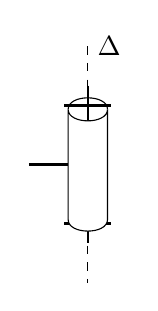
\begin{tikzpicture}
    \draw[thick] (0,0) -- (0.5, 0);
    \draw (0.5, 0.7) to[out=90, in=90] (1, 0.7);
    \draw[thick] (0.75, 1) -- (0.75, -1);
    \draw[dashed] (0.75, 1.5) node[right]{$\Delta$}  -- (0.75, -1.5);
    \draw[thick] (0.45, 0.75) -- (1.05, 0.75);
    \draw[thick] (0.45, -0.75) -- (1.05, -0.75);
    \draw[fill=white] (0.5, -0.7) -- (0.5,0.7) to[out=-90, in=-90] (1,0.7) -- (1, -0.7) to[out=-90, in=-90](0.5,-0.7);
  \end{tikzpicture}
  \captionof{figure}{Liaison pivot}
\end{center}

\section{Théorème du moment cinétique}%
\label{sec:theoreme_du_moment_cinetique}

\subsection{Théorème du moment cinétique}%
\label{sub:theoreme_du_moment_cinetique}
\begin{loi}{Théorème du moment cinétique}
  Dans un référentiel galiléen, la variation du moment cinétique d'un point matériel $M$ par rapport à un point fixe $O$ est égal à la somme des moments des forces appliquées à $M$. 
  \begin{equation}
    \dt{\vv*{L}{O}(M)} = \sum_i \vv*{\M}{O}(\vv*{F}{i})
  \end{equation}
\end{loi}
On peut le démontrer à partir du principe fondamental de la dynamique :
\begin{align}
  \vv*{L}{O}(M) = \vv{OM}\wedge \vv{p} \Leftrightarrow \dt{\vv*{L}{O}(M)} = \underbrace{\dt{\vv{OM}}\wedge\vv{p}}_{\vv{v}\wedge \vv{p}=0} + \vv{OM}\wedge \dt{\vv{p}} = \sum_i \vv{OM}\wedge\vv*{F}{i} = \sum_i \vv*{\M}{O}(\vv*{F}{i})
\end{align}

Si la somme des moments de forces appliquées à un point matériel est nulle, alors le moment cinétique du point matériel est conservé.

\subsection{Loi scalaire du moment cinétique pour un solide}%
\label{sub:loi_scalaire_du_moment_cinetique_pour_un_solide}

Le théorème du moment cinétique s'étend facilement à un système de points matériels et donc à un solide. Pour un solide en rotation autour d'un axe fixe $\Delta$ , on peut projeter cette relation sur l'axe orienté $\Delta$.

\begin{loi}{Loi scalaire du moment cinétique}
  Pour un solide en rotation autour d'un axe fixe $\Delta$ dans un référentiel galiléen, la variation du moment cinétique du solide par rapport à l'axe $\Delta$ est égale à la somme des moments des forces appliquées par rapport à $\Delta$. 
  \begin{equation}
    \dt{L_\Delta} = \sum_i \M_\Delta(\vv*{F}{i})
  \end{equation}
\end{loi}

\subsection{Application au pendule pesant}%
\label{sub:application_au_pendule_pesant}

Un pendule pesant est constitué d'un solide $S$ pouvant tourner librement (liaison pivot) autour d'un axe vertical $\Delta$. Le solide étant soumis à son poids et à la réaction de l'axe.

\begin{center}
  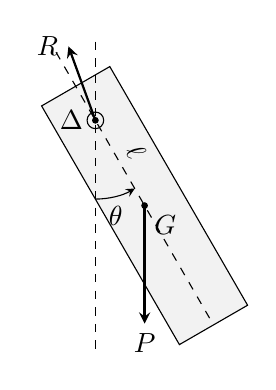
\begin{tikzpicture}
  %tikz meca
    \draw[rotate=30, fill=gray!10] (-0.5,0.5) rectangle (0.5, -3);
    \draw[fill=black] (0,0) coordinate (O) circle(1pt);
    \draw (O) circle(3pt) node[xshift=-1pt, left] {$\Delta$}; 
    \draw[fill] (O) ++ (-60:1.25) circle(1pt) coordinate(G) node[below right]{$G$};
    \draw[thick, -stealth](G) -- ++(0,-1.5) node[below] {$\vv{P}$ };
    \draw[thick, -stealth](O) -- ++(110:1) node[left] {$\vv{R}$ };
    \draw[dashed](0, 1) -- (0, -3);
    \draw[dashed] (O) ++ (120:1) -- ++(-60:4) node[pos=0.4, sloped, above]{$\ell$ };
    \draw[-stealth] (O) ++ (-90:1) arc (-90:-60:1) node[midway, below]{$\theta$ };
  \end{tikzpicture}
\captionof{figure}{Pendule pesant}
\label{fig:pendule_pesant}
\end{center}
On note $J_\Delta$ le moment d'inertie de $S$ par rapport à $\Delta$ et $\ell$ la distance entre $G$ et l'axe $\Delta$. 

On applique la loi du moment cinétique au solide $S$ : 
\begin{equation}
  \dt{L_\Delta} = \M_\Delta(\vv{P}) + \underbrace{\M_\Delta(\vv{R})}_{=0} = -mg\ell\sin(\theta)
\end{equation}
car le bras de levier de la force $\vv{P}$ est $\ell\sin(\theta)$ et le poids fait tourner le solide dans le \og{}mauvais sens\fg{} par rapport à l'orientation de $\Delta$. Comme de plus on a $L_\Delta = J_\Delta \dot{\theta}$, on obtient l'équation 
\begin{eqencadre}
  \ddot{\theta}+\frac{mg\ell}{J_\Delta}\sin(\theta) = 0
  \label{eq:pendule_nl}
\end{eqencadre}
C'est sensiblement la même équation que celle obtenue pour un pendule simple. Elle est non linéaire et difficile à résoudre. Mais pour de petites oscillations ($\theta\ll 1$) on peut linéariser le sinus et on obtient:
\begin{eqencadre}
  \ddot{\theta} + \frac{mg\ell}{J_\Delta}\theta = 0
\end{eqencadre}
qui est l'équation d'un oscillateur harmonique de pulsation propre $\omega_0 = \sqrt{\frac{mg\ell}{J_\Delta}}$. Dans ce cas, on connait la solution générale, qui est $\theta(t) = A\cos(\omega_0t + \varphi)$, et le portrait de phase est une ellipse. 

Pour des oscillations de plus grande amplitude, il faut résoudre l'équation différentielle~\ref{eq:pendule_nl} numériquement pour déterminer le mouvement du pendule. On peut notamment montrer que dans ce cas, la période d'oscillation dépend de l'amplitude des oscillations (non isochronisme des oscillations)

\begin{minted}{python}
import numpy as np
import matplotlib.pyplot as plt
import scipy.integrate

# Équation différentielle à résoudre
def eq(t, y):
    theta, theta_p = y
    w0 = 2
    return [theta_p, -w0**2*np.sin(theta)]
    
# Détermine la période d'un signale périodique
def trouve_periode(s, t):
    # Détermine le premier croisement de 0
    i=0
    while s[i]>0:
        i+=1
    # Interpolation linéaire pour trouver l'intersection avec 0
    # C'est plus précis que de prendre t1=t[i] ou t1=t[i+1]
    t1 = (s[i+1]*t[i] - s[i]*t[i+1])/(s[i+1] - s[i]) 
    # Oublie un passage par 0 (car 2 passage par 0 par période)
    while s[i]<0:
        i+=1
    # Passage suivant par 0
    while s[i]>0:
        i+=1
    # Interpolation linéaire pour trouver l'intersection avec 0
    t2 = (s[i+1]*t[i] - s[i]*t[i+1])/(s[i+1] - s[i]) 
    return t2-t1

t0 = []
T = []
for theta0 in np.linspace(0.1, 0.7*np.pi, 50):
    T_MAX = 10
    y0 = [theta0, 0]
    t = [0, T_MAX]
    t_ech = np.linspace(0, T_MAX, 500)
    sol = scipy.integrate.solve_ivp(eq, t, y0, t_eval=t_ech)
    t0.append(theta0)
    T.append(trouve_periode(sol.y[0], sol.t))
plt.plot(t0, T,'*')
plt.show()
\end{minted}

\begin{center}
  \begin{tikzpicture}
   \begin{axis}[
     xmin=0,
     xmax=0.7*pi,
     xlabel = $\theta_0$ (\si{\radian}),
     ylabel = Période (\si{\s}),
     %xtick = {0, pi/2, pi}, 
     %xticklabels={0, $\pi/2$, $\pi$},    
     minor x tick num=1,
     minor y tick num=1,
     grid=both,
 ] 
   \addplot[no marks,smooth, thick] table[x index=0, y index=1] {data/periode_pendule.csv};
     
   \end{axis} 
  \end{tikzpicture}
  \captionof{figure}{Période d'oscillation du pendule en fonction de son amplitude}\label{fig:periode}
\end{center}
%\begin{center}
  %\begin{tikzpicture}
   %\begin{axis}[
     %xmin=-4*pi,
     %xmax=4*pi,
     %xlabel = $\theta$ (\si{\radian}),
     %minor x tick num=1,
     %minor y tick num=1,
     %ylabel = $\dot{\theta}$ (\si{\radian\per\second}),
     %xtick = {-4*pi, -2*pi, 0, 2*pi, 4*pi}, 
     %xticklabels={$-4\pi$, $-2\pi$, 0, $2\pi$, $4\pi$},    
     %grid=both,
 %] 
   %\addplot[no marks,smooth] table[x index=0, y index=1] {data/portrait_phase_pendule.csv};
   %\addplot[no marks,smooth] table[x index=2, y index=3] {data/portrait_phase_pendule.csv};
   %\addplot[no marks,smooth] table[x index=4, y index=5] {data/portrait_phase_pendule.csv};
   %\addplot[no marks,smooth] table[x index=6, y index=7] {data/portrait_phase_pendule.csv};
   %\addplot[no marks,smooth] table[x index=8, y index=9] {data/portrait_phase_pendule.csv};
   %\addplot[no marks,smooth] table[x index=10, y index=11] {data/portrait_phase_pendule.csv};
   %\addplot[no marks,smooth] table[x index=12, y index=13] {data/portrait_phase_pendule.csv};
     
   %\end{axis} 
  %\end{tikzpicture}
  %\captionof{figure}{Portrait de phase du pendule pesant pour différentes amplitudes d'oscillation}\label{fig:portrait_phase}
%\end{center}


%On remarque qu'au dessus d'une certaine vitesse angulaire maximale, on passe d'un mouvement d'oscillations à un mouvement de révolution autour de l'axe $\Delta$. 
On voit bien sur ce graphique qu'à faible amplitude, la période ne dépend pas de l'amplitude (tangente horizontale en $0$) alors que lorsque l'amplitude augmente, la période augmente.



\section{Aspect Énergétique}%
\label{sec:aspect_energetique}

\subsection{Énergie cinétique d'un solide en rotation}%
\label{sub:energie_cinetique_d_un_solide_en_rotation}
L'énergie cinétique d'un solide en rotation est la somme des énergies cinétiques des points qui le composent. La vitesse d'un point $M_i$ situé à une distance $r_i$ de l'axe de rotation $\Delta$ est $v_i = r_i \omega$, où $\omega$ est la vitesse angulaire de rotation du solide.

L'énergie cinétique totale du solide s'écrit donc comme
\begin{equation}
  E_c = \sum_i \frac{1}{2}m_i v_i^2 = \frac{1}{2}\sum_i m_i r_i^2\omega^2 = \frac{1}{2}\omega^2\underbrace{\sum_i m_i r_i^2}_{J_\Delta}
\end{equation}
On reconnait l'expression de $J_\Delta$ et l'énergie cinétique d'un solide en rotation à la vitesse angulaire $\omega$ autour d'un axe fixe $\Delta$ est
\begin{eqencadre}
  E_c = \frac{1}{2}J_\Delta \omega^2
\end{eqencadre}


\subsection{Loi de l'énergie cinétique}%
\label{sub:loi_de_l_energie_cinetique}
Nous allons établir l'équivalent du théorème de l'énergie cinétique pour un solide en rotation autour d'un axe fixe. On part du théorème du moment cinétique 
\begin{equation}
  \dt{L_\Delta} = \sum_i \M_\Delta(\vv*{F}{i}) \Leftrightarrow J_\Delta \dot{\omega} = \sum_i \M_\Delta(\vv*{F}{i})
\end{equation}
En multipliant chaque côté de l'équation par $\omega$, on obtient 
\begin{equation}
  J_\Delta  \omega \dot{\omega} = \sum_i  \M_\Delta(\vv*{F}{i}) \omega \Leftrightarrow \dt{}\underbrace{\left(\frac{1}{2}J_\Delta \omega^2\right)}_{E_c} = \sum_i \underbrace{\M_\Delta(\vv*{F}{i})\omega}_{P_i}
\end{equation}

\begin{loi}{Loi de l'énergie cinétique}
  Pour un solide en rotation autour d'un axe fixe $\Delta$ dans un référentiel galiléen, on a 
  \begin{equation}
    \dt{E_c} = \sum_i P_i
  \end{equation}
  où $P_i = \M_\Delta(\vv*{F}{i})\omega$ est la puissance fournie au solide par la force $\vv*{F}{i}$.  
\end{loi}

On peut appliquer cette loi pour retrouver l'équation du mouvement du pendule pesant (voir figure~\ref{fig:pendule_pesant}). Avec $E_c = \frac{1}{2}J_\Delta \dot{\theta}^2$, $\M_\Delta(\vv{P}) = -mg\ell\sin(\theta)$ et $\M_\Delta(\vv{R})=0$.   

On a donc
\begin{equation}
\frac{1}{2}J_\Delta  \dt{\dot{\Theta}^2} = -mg\ell\sin(\theta)\times \dot{\theta} \Leftrightarrow \frac{1}{2}J_\Delta \times 2 \ddot{\theta} \dot{\theta} = -mg\ell\sin(\theta)\dot{\theta} \Leftrightarrow J_\Delta \ddot{\theta} = -mg\ell\sin(\theta)
\end{equation}

Et on retrouve bien la même équation que dans la partie~\ref{sec:theoreme_du_moment_cinetique}\ref{sub:application_au_pendule_pesant}. Heureusement !


\end{document}
